\documentclass[17pt,twoside]{extarticle}
\usepackage[a4paper, margin=1.7cm]{geometry}
\usepackage{fancyhdr}
\pagestyle{fancy}
\usepackage{graphicx}
\usepackage{lmodern}
\usepackage{amssymb,amsmath}
\usepackage{ifxetex,ifluatex}
\usepackage{fixltx2e} % provides \textsubscript
\ifnum 0\ifxetex 1\fi\ifluatex 1\fi=0 % if pdftex
  \usepackage[T1]{fontenc}
  \usepackage[utf8]{inputenc}
\else % if luatex or xelatex
  \ifxetex
    \usepackage{mathspec}
    \usepackage{xltxtra,xunicode}
  \else
    \usepackage{fontspec}
  \fi
  \defaultfontfeatures{Mapping=tex-text,Scale=MatchLowercase}
  \newcommand{\euro}{€}
\fi
% use upquote if available, for straight quotes in verbatim environments
\IfFileExists{upquote.sty}{\usepackage{upquote}}{}
% use microtype if available
\IfFileExists{microtype.sty}{%
\usepackage{microtype}
\UseMicrotypeSet[protrusion]{basicmath} % disable protrusion for tt fonts
}{}
\ifxetex
  \usepackage[setpagesize=false, % page size defined by xetex
              unicode=false, % unicode breaks when used with xetex
              xetex]{hyperref}
\else
  \usepackage[unicode=true]{hyperref}
\fi
\hypersetup{breaklinks=true,
            bookmarks=true,
            pdfauthor={},
            pdftitle={},
            colorlinks=true,
            citecolor=blue,
            urlcolor=blue,
            linkcolor=magenta,
            pdfborder={0 0 0}}
\urlstyle{same}  % don't use monospace font for urls
\setlength{\parindent}{0pt}
\setlength{\parskip}{6pt plus 2pt minus 1pt}
\setlength{\emergencystretch}{3em}  % prevent overfull lines
\setcounter{secnumdepth}{0}

\setmainfont{Garamond Premier Pro}

\title{SHAKE-SPEARES ORACLES}
\author{Plum Village}
\date{2015}

\fancypagestyle{plain}
\fancyhead{}
\fancyhead[C]{\slshape SHAKE-SPEARES ORACLES}
\fancyhead[LE]{\thepage}
\fancyhead[RO]{\thepage}
\headheight = 37pt
\fancyfoot{}

\begin{document}

\begin{figure}[htbp]
     \centering
     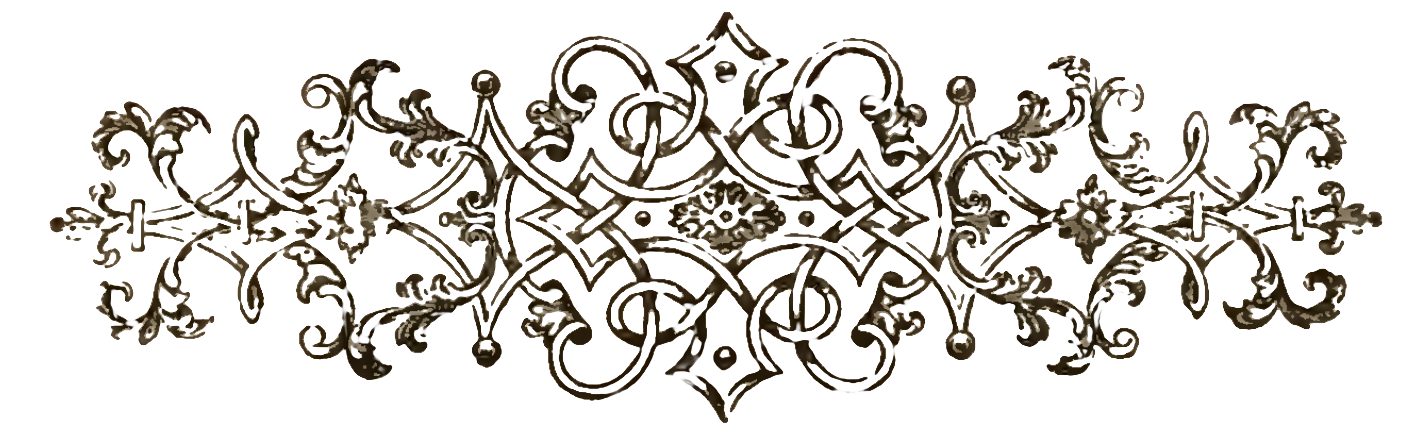
\includegraphics[width=15.5cm]{images/frontispiece.png}
\end{figure}

\begin{enumerate}
\item
  To swim, to dive into the fire, to ride on the curled
  clouds,\footnote{The Tempest 1.2: Ariel. Miraculous action, as quick
    as thought.}\\Whose speechless song being many, seems one.\footnote{Sonnet
    8. ``Seeming'' changed to ``seems''. Thunder is the speechless song
    of clouds.}
\item
  Time doth transfix the flourish set on youth,\footnote{Sonnet 60.
    \textbf{doth} does \textbf{transfix} pierce \textbf{flourish}
    bloom/adornment}\\Which bounteous gift thou shouldst in bounty
  cherish.\footnote{Sonnet 11. \textbf{thou shouldst} you should
    \textbf{in bounty} generously}
\item
  Be collected; no more amazement. Tell your piteous heart:\footnote{The
    Tempest 1.2: Prospero. \textbf{collected} calm, composed
    \textbf{amazement} fear/wonder}\\Thou art thy mother's glass, and
  she in thee.\footnote{Sonnet 3. \textbf{glass} mirror \textbf{thee}
    you. You are your mother's reflection.}
\item
  So, ere you find where light in darkness lies,\footnote{Love's Labour
    Lost 1.1: Berowne. \textbf{ere} before}\\Gentle breath of yours my
  sails must fill.\footnote{The Tempest, Epilogue: Prospero}
\item
  Grant, if thou wilt, thou art beloved of many,\footnote{Sonnet 10.}\\Both
  in your form and nobleness of mind.\footnote{Richard III 3.7:
    Buckingham}
\item
  Now my charms are all o'erthrown,\footnote{The Tempest Epilogue:
    Prospero. ``Charms'' here means ``spells'' or ``enchantments.''}\\Begot
  of nothing but vain fantasy.\footnote{Romeo and Juliet 1.4: Mercutio.
    ``I talk of dreams.''}
\item
  Look, whom she best endow'd she gave thee more;\footnote{Sonnet 11.
    ``She'' here is Nature.}\\Our fancies are more giddy and
  unfirm.\footnote{Twelfth Night 2.4: Duke Orsino. Here he notes the
    unsteadiness of man's desires.}
\item
  Sap checked with frost and lusty leaves quite gone,\footnote{Sonnet 5.
    Trees in winter.}\\Courage and hope both teaching him the
  practice.\footnote{Twelfth Night 1.2: Captain. He reassures Viola that
    her brother may have saved himself from drowning.}
\item
  Rough winds do shake the darling buds of May.\footnote{Sonnet 18.
    Inclement weather precedes summer.}\\I'll kneel down, and ask of
  thee forgiveness.\footnote{King Lear 5.3: King Lear. He vows to begin
    anew with his daughter Cordelia for having judged her wrongly.}
\item
  Hourly joys be still upon you!\footnote{The Tempest 4.1: Juno}\\And
  frame your mind to mirth and merriment.\footnote{The Merchant of
    Venice 1.2: Messenger}
\item
  The moon new-bent in heaven, shall behold the night\footnote{A
    Midsummer Night's Dream 1.1: Hippolyta. The moon overlooking the
    world at night.}\\That has such people in't!\footnote{The Tempest
    5.1: Miranda. She wonders at Alonso's retinue upon his reunion with
    Ferdinand, after being raised by Prospero apart from humanity.}
\item
  And having climb'd the steep-up heavenly hill,\footnote{Sonnet 7. The
    sun rising.}\\Fortune, good night: smile once more: turn thy
  wheel!\footnote{King Lear 2.2: Kent. He has been put in stocks by
    Cornwall and Regan, Lear's daughter.}
\item
  Beauty o'ersnow'd and bareness every where\footnote{Sonnet 5. The
    earth at winter.}\\Thaws and resolves itself into a dew.\footnote{Hamlet,
    Prince of Denmark 1.2: Hamlet. Added ``s'' to thaw and resolve.}
\item
  Their eyes do offices of truth, their words are natural breath,
  \footnote{The Tempest 5.1: Prospero}\\All dedicated to closeness and
  the bettering of my mind.\footnote{The Tempest 1.2: Prospero.}
\item
  Sound me from my lowest note to the top of my compass:\footnote{Hamlet,
    Prince of Denmark 3.2: Hamlet. He charges Guildenstern with trying
    to play upon him to discover the root of his discontent.}\\My heart
  is true as steel.\footnote{A Midsummer Night's Dream 2.1: Helena. She
    professes the steadfastness of her love for Demetrius.}
\item
  Thy self thy foe, to thy sweet self too cruel;\footnote{Sonnet 1.}\\I
  am sure care's an enemy to life.\footnote{Twelfth Night 1.3: Sir Toby
    Belch. He feels his niece Olivia should be free of the sorrow caused
    by her brother's death.}
\item
  Sermons in stones, and good in everything---\footnote{As You Like It
    2.1: Duke Senior}\\And therefore sit you down in
  gentleness.\footnote{As You Like It 2.7: Duke Senior}
\item
  Have more than thou showest, speak less than thou knowest,\footnote{The
    Tempest 2.1: Antonio.}\\Nor lose possession of that fair thou
  ow'st.\footnote{Sonnet 18. For ``thou ow'st'' read ``you own,''
    meaning that fair which is yours.}
\item
  What seest thou else in the dark backward and abysm of time?\footnote{The
    Tempest 1.2: Prospero. He asks Miranda to see what she remembers of
    her past.}\\So full of shapes is fancy that it alone is high
  fantastical.\footnote{Twelfth Night 1.1: Duke Orsino. He sees the
    fleeting nature of romantic love.}
\item
  To give away yourself, keeps yourself still.\footnote{Sonnet 16.}\\Make
  me a willow cabin at your gate.\footnote{Twelfth Night 1.5: Viola}
\item
  Those be rubies, fairy favors;\footnote{A Midsummer Night's Dream 2.1:
    Fairy. He describes the spots on cowslips.}\\They sparkle still the
  right Promethean fire.\footnote{Love's Labour Lost: 4.3.
    \textbf{still\ldots{}fire} continually with the heavenly fire stolen
    by Prometheus.}
\item
  Men must endure their going hence, even as their coming
  hither.\footnote{King Lear 5.2: Edgar. He speaks these lines to
    Gloucester after learning that Cordelia has lost the battle in order
    to rouse him. No coming, no going. Present moment.}\\I am a fool to
  weep at what I am glad of.\footnote{The Tempest 2.1: Miranda.}
\item
  Get thee to a nunnery:\footnote{Hamlet, Prince of Denmark 3.1: Hamlet.
    Seeing his destructive emotions and afraid for Ophelia's wellbeing,
    he pushes her away.}\\A contract of true love to
  celebrate.\footnote{The Tempest 4.1: Iris. Spirits celebrate
    Ferdinand's winning of Miranda's hand.}
\item
  If music be the food of love, play on,\footnote{Twelfth Night 1.1:
    Orsino.}\\And let this world no longer be a stage.\footnote{Henry
    the Fourth, Part 2 1.1: Northumberland.}
\item
  A man may see how this world goes with no eyes. Look with thine
  ears:\footnote{King Lear 4.6: King Lear. To the blinded Gloucester.}\\The
  murmuring surge, that on the unnumber'd idle pebbles chafes.\footnote{King
    Lear 4.6: Edgar. To Gloucester.}
\item
  And manifest experience had collected\footnote{All's Well That Ends
    Well 1.3: Helena.}\\Of drops that sacred pity hath
  engend'red.\footnote{As You Like It 2.7: Duke Senior.}
\item
  How beauteous mankind is! O brave new world,\footnote{The Tempest 5.1:
    Miranda. On seeing her betrothed Ferdinand's father Alonso and his
    retinue.}\\Merrily, merrily, shall I live now.\footnote{The Tempest
    5.1: Ariel. On learning he will soon be freed from his service to
    Prospero.}
\item
  These our actors, as I foretold you, were all spirits and\footnote{The
    Tempest 4.1: Prospero. Explaining his magic arts to Ferdinand.}\\Do
  make me give the lie to my true sight.\footnote{Sonnet 150. ``To''
    changed to ``do.'' Stop seeing the truth.}
\item
  With the help of your good hands\footnote{The Tempest 5.1: Prospero.
    Hands that release him from his bonds.} all things in common
  nature\\Should produce without sweat or endeavour.\footnote{The
    Tempest 2.1: Gonzalo.}
\item
  And some donation freely to estate\footnote{The Tempest 4.1: Iris.}\\Under
  the blossom that hangs on the bough.\footnote{The Tempest 5.1: Ariel.}
\item
  Sounds and sweet airs, that give delight and hurt not:\footnote{The
    Tempest 3.2: Caliban.}\\In a cowslip's bell I lie.\footnote{The
    Tempest 5.1: Ariel.}
\item
  But that the dread of something after death\footnote{Hamlet, Prince of
    Denmark 3.1: Hamlet.}\\It droppeth as the gentle rain from
  heaven.\footnote{The Merchant of Venice 4.1: Portia. She speaks of the
    quality of mercy.}
\item
  And ye that on the sands with printless foot\\Do chase the ebbing
  Neptune---\footnote{Richard III 5.5: Henry, Earl of Richmond.}\\O, let
  me see thee walk! Thou dost not halt.\footnote{Henry IV, Part 1 2.4:
    Falstaff.}
\item
  But, like a cloistress, she will veiled walk\footnote{Twelfth Night
    1.1: Valentine. To Duke Orsino on Olivia's mourning of her brother's
    death.}\\Out of the jaws of death.\footnote{Twelfth Night 3.4:
    Antonio.}
\item
  As there is sense in truth and truth in virtue,\footnote{Measure For
    Measure 5.1: Mariana.}\\Joy, gentle friends, joy and fresh days of
  love accompany your hearts!\footnote{A Midsummer Night's Dream 5.1:
    Theseus.}
\item
  For who would bear the whips and scorns of time,\footnote{Hamlet,
    Prince of Denmark 3.1: Hamlet.}\\And kiss the lips of unacquainted
  change?\footnote{King John 3.4: Pandulph.}
\item
  Often have you heard that told:\footnote{The Merchant of Venice 2.7:
    Morocco.} Wherefore are these things hid?\\Wherefore have these
  gifts a curtain before 'em?\footnote{Twelfth Night 1.3: Sir Toby
    Belch.}
\item
  And summer's lease hath all too short a date:\footnote{Sonnet 18.}\\The
  hour's now come; the very minute bids thee ope thine ear.\footnote{The
    Tempest 1.2: Prospero. He reveals to Miranda her past. ``Ope'' is
    ``open,'' ``thine'' is ``your.''}
\item
  I am all the daughters of my father's house, and all the brothers
  too.\footnote{Twelfth Night 2.4: Viola.}\\O spirit of love! how quick
  and fresh art thou.\footnote{Twelfth Night 1.1: Duke Orsino.}
\item
  And enterprises of great pith and moment\footnote{Hamlet, Prince of
    Denmark 3.1: Hamlet. Our projects, our cows, etc..}\\Are melted into
  air, into thin air.\footnote{The Tempest 4.1: Prospero. What becomes
    of his conjured spirits.}
\item
  O, swear not by the moon, the inconstant moon,\footnote{Romeo and
    Juliet 2.2: Juliet. Her response to Romeo's avowals.}\\If it be not
  now, yet it will come: the readiness is all.\footnote{Hamlet, Prince
    of Denmark 5.2: Hamlet. Before dueling with Laertes.}
\item
  And fearless minds climb soonest unto crowns\footnote{Henry VI, Part
    III 4.7: Gloucester. \textbf{crowns} awakening}\\That show, contain
  and nourish all the world.\footnote{Love's Labour Lost 4.3: Biron.}
\item
  Youth's a stuff will not endure;\footnote{Twelfth Night 1.2: Viola.}\\Out
  of that no hope what great hope have you!\footnote{Hamlet, Prince of
    Denmark 1.2: Hamlet. Interpretation: A disguise or a self only leads
    to weariness.}
\item
  And thus the native hue of resolution\footnote{Hamlet, Prince of
    Denmark 3.1: Hamlet.}\\Lies rich in virtue and unmingled.\footnote{Troilus
    and Cressida 1.3: Agamemnon.}
\item
  Happiness courts thee in her best array\footnote{Romeo and Juliet 3.3:
    Friar John.}\\And joy comes well in such a needy time.\footnote{Romeo
    and Juliet 3.5: Juliet.}
\item
  Nature's bequest gives nothing but doth lend;\footnote{Sonnet 4.}\\Thy
  truth, then, be thy dower.\footnote{King Lear 1.1: King Lear. Despite
    Cordelia's honesty, Lear does not perceive her faithfulness to him.
    These verses incite us to engage with truth as a test of faith,
    leaving behind the dower of possessions.}
\item
  Study is like the heaven's glorious sun,\footnote{Love's Labour Lost
    1.1: Berowne. True study brings clarity.}\\Which touch'd the very
  virtue of compassion in thee.\footnote{The Tempest 1.2: Prospero.}
\item
  Uttering such dulcet and harmonious breath\footnote{A Midsummer
    Night's Dream 2.1: Oberon.}\\That long have frown'd upon their
  enmity!\footnote{Richard III 5.5: Richmond. Brotherhood and peace to
    succeed strife.}
\item
  Give me your hands, if we be friends;\footnote{A Midsummer Night's
    Dream 5.1: Puck.}\\We are such stuff as dreams are made
  on.\footnote{The Tempest 4.1: Prospero. On the insubstantiality of
    phenomenal objects.}
\item
  And nothing 'gainst Time's scythe can make defence---\footnote{Sonnet
    12. Impermanence.}\\Herein lives wisdom, beauty and
  increase.\footnote{Sonnet 11. Touching impermanence we get wisdom, and
    our love increases.}
\item
  I must go seek some dewdrops here;\footnote{A Midsummer Night's Dream
    2.1: Fairy.}\\It blesseth him that gives and him that
  takes.\footnote{The Merchant of Venice 4.1: Portia. On mercy
    (compassion).}
\item
  I put you to the use of your own virtues.\footnote{All's Well That
    Ends Well 5.1: Helena.}\\All things are ready, if our minds be
  so.\footnote{Henry V 4.3: King Henry}
\item
  Now stand you on the top of happy hours,\footnote{Sonnet 16.}\\Against
  the stormy gusts of winter's day.\footnote{Sonnet 13.}
\item
  Let gentleness my strong enforcement be\footnote{As You Like It 2.7:
    Orlando}\\To take a new acquaintance of thy mind.\footnote{Sonnet
    77.}
\item
  To take arms against a sea of troubles, and by opposing end
  them?\footnote{Hamlet, Prince of Denmark 3.1: Hamlet.}\\Let it not
  enter in your mind of love.\footnote{Merchant of Venice 2.8: Salerio.}
\item
  These most brisk and giddy-paced times:\footnote{Twelfth Night 2.4:
    Duke Orsino.}\\Is man no more than this? Consider him
  well.\footnote{King Lear 3.4: King Lear.}
\item
  Who with thy saffron wings upon my flowers\footnote{The Tempest 4.1:
    Ceres.}\\Calls back the lovely April of her prime:\footnote{Sonnet
    3.} the form of my intent.\footnote{Twelfth Night 1.2: Viola.
    Beginner's mind, aspiration.}
\item
  It is a wise father that knows his own child,\footnote{The Merchant of
    Venice 2.2: Launcelot.}\\Like to a double cherry, seeming parted,
  but yet an union in partition.\footnote{A Midsummer Night's Dream 3.2:
    Helena.}
\item
  In action how like an angel! In apprehension how like a god,
  \footnote{Hamlet, Prince of Denmark 2.2: Hamlet. He speaks of man.}\\That
  the rude sea grew civil at her song.\footnote{A Midsummer Night's
    Dream 2.1: Oberon. Of a mermaid on a dolphin's back.}
\item
  Gaze where you should, and that will clear your sight.\footnote{Comedy
    of Errors 3.2: Luciana.}\\Enrich the time to come with smooth-fac'd
  peace.\footnote{Richard III 5.5: Henry, Earl of Richmond.}
\item
  The slings and arrows of outrageous fortune---\footnote{Hamlet, Prince
    of Denmark 3.1: Hamlet. Suffering resulting from past actions.}\\These
  blessed candles of the night.\footnote{The Merchant of Venice 5.1:
    Bassanio. The stars.}
\item
  O, from what power hast thou this powerful might,\footnote{Sonnet 150.}\\By
  chance or nature's changing course untrimm'd?\footnote{Sonnet 18. The
    insight of impermanence gives us power over our lives.}
\item
  Rise from the ground like feathered Mercury,\footnote{Henry IV, Part 1
    4.1: Vernon.}\\Then to the elements be free, and fare thou
  well!\footnote{The Tempest, 5.1: Prospero.}
\item
  The constancy and virtue of your love---\footnote{Sonnet 117}\\Diffusest
  honey-drops, refreshing showers.\footnote{The Tempest 4.1: Ceres.}
\item
  For never-resting time leads summer on---\footnote{Sonnet 5. Time here
    is impermanence.}\\The wheel is come full circle: I am
  here.\footnote{King Lear 5.3: Edmund. On discovering his half-brother
    Edgar.}
\item
  But how is it that this lives in thy mind,\footnote{The Tempest 1.2:
    Prospero}\\The undiscover'd country from whose bourn no traveller
  returns? \footnote{Hamlet, Prince of Denmark 3.1: Hamlet. What is
    beyond death.}
\item
  They are the books, the arts, the academes---\footnote{Love's Labour
    Lost: 4.3. \textbf{academes} academies. They put their life into
    books, arts, or intellectual knowledge.}\\And I serve the fairy
  queen.\footnote{A Midsummer Night's Dream 2.1: Fairy.}
\item
  Smooth runs the water where the brook is deep.\footnote{The Tempest,
    Epilogue: Prospero.}\\What stronger breastplate than a heart
  untainted?\footnote{The Tempest 2.1: Gonzalo.}
\item
  Then wisely, good sir, weigh our sorrow with our comfort,\footnote{The
    Tempest 2.1: Gonzalo.}\\That ebb and flow by the moon.\footnote{King
    Lear 5.3: King Lear.}
\item
  All that glisters is not gold. To plainness honour's bound\footnote{The
    Merchant of Venice 2.7.}\\When majesty falls to folly.\footnote{King
    Lear 1.1: Kent. King Lear is caught in the wrong view that his
    daughter Cordelia is not grateful to him. Kent, knowing her
    faithfulness, tries to intervene.}
\item
  Think'st thou I'd make a life of jealousy?\footnote{Othello 3.3:
    Othello. Iago plants false seeds in Othello of his wife's
    unfaithfulness. Othello says he will not live in jealousy.}\\The
  quality of mercy is not strain'd.\footnote{The Merchant of Venice 4.1:
    Portia. Compassion frees us from the bonds of jealousy, and it is
    not difficult at all.}
\item
  O heaven, O earth, bear witness to this sound,\footnote{The Tempest
    2.1: Miranda.}\\As full of spirit as the month of May.\footnote{Henry
    IV, Part 1 4.1: Vernon.}
\item
  When I consider every thing that grows\\Holds in perfection but a
  little moment---\footnote{Sonnet 15.}\\Pray you, tread softly, that
  the blind mole may not hear a foot fall.\footnote{The Tempest 4.1:
    Caliban.}
\item
  With gentle conference, soft and affable,\footnote{Taming of the Shrew
    2.1: Petruchio.}\\Let your indulgence set me free.\footnote{The
    Tempest, Epilogue: Prospero.}
\item
  Light, seeking light, doth light of light beguile;\footnote{Love's
    Labour Lost 1.1: Berowne. \textbf{Light} i.e., eyes \textbf{light}
    enlightenment \textbf{light\ldots{}beguile} we are cheated out of
    enlightenment by excessive searching}\\Now let not Nature's hand
  keep the wild flood confin'd!\footnote{Henry IV, Part 2 1.1:
    Northumberland.}
\item
  True, I talk of dreams,\footnote{Romeo and Juliet 1.4: Mercutio. This
    follows Romeo's interruption on his depiction of Queen Mab, who
    tempts men and women with desires in their sleep.} for there is
  nothing\\Either good or bad, but thinking makes it so.\footnote{Hamlet,
    Prince of Denmark 2.2: Hamlet. In conversation with Guildenstern he
    sees Denmark as a prison, but recognizes that this it the product of
    his own thinking.}
\item
  What's in a name? that which we call a rose\footnote{Romeo and Juliet
    2.2: Juliet. She sees the illusory nature of the world of name and
    form.}\\Being once display'd doth fall that very hour.\footnote{Twelfth
    Night 2.4: Orsino.}
\item
  O, if you but knew how you the purpose cherish!\footnote{The Tempest,
    Epilogue: Prospero.}\\If all were minded so, the times should
  cease.\footnote{Sonnet 11.}
\item
  What is love? 'tis not hereafter,\footnote{Twelfth Night 2.3: Feste.}\\And
  being frank she lends to those are free.\footnote{Sonnet 4.}
\item
  What's to come is still unsure;\footnote{Twelfth Night 2.3: Feste.}
  what's past is prologue.\footnote{The Tempest 2.1: Antonio.}\\Present
  mirth hath present laughter.\footnote{Twelfth Night 2.3: Feste.}
\item
  And the moon changes even as your mind,\footnote{The Taming of the
    Shrew 4.5: Katherina.}\\But thy eternal summer shall not
  fade.\footnote{Sonnet 18.}
\item
  I, thus neglecting worldly ends,\footnote{The Tempest 1.2: Prospero.}\\Play
  out the play.\footnote{Henry IV, Part 1 2.4: Falstaff.}
\item
  Continue still in this so good a mind,\footnote{Henry VI, Part II 4.9:
    King Henry.}\\Wherein it finds a joy above the rest.\footnote{Sonnet
    91.}
\item
  To forswear the full stream of the world\\And to live in a nook merely
  monastic\footnote{As You Like It 3.2: Rosalind.}\\And by my body's
  action teach my mind.\footnote{Coriolanus 3.2: Coriolanus.}
\item
  Defer no time, delays have dangerous ends;\footnote{Henry VI, Part 1:
    Alençon.}\\Thou shalt be as free as mountain winds.\footnote{The
    Tempest 1.2: Prospero.}
\item
  Understanding begins to swell \footnote{The Tempest 5.1: Prospero.} by
  prayer, which pierces so\\That it assaults mercy itself, and frees all
  faults.\footnote{The Tempest, Epilogue: Prospero.}
\item
  As it is a spare life, look you, it fits my humour well,\footnote{As
    You Like It 3.2: Touchstone.}\\With smiling plenty, and fair
  prosperous days!\footnote{Richard III 5.5: Richmond.}
\item
  Th'endeavour of this present breath may buy\footnote{Love's Labour
    Lost 1.1: King. \textbf{endeavour} attempt to achieve a goal}\\The
  very lifeblood of our enterprise.\footnote{Henry IV, Part 1 4.1:
    Hotspur.}
\item
  But I will tarry; the fool will stay, and let the wise man
  fly,\footnote{King Lear 2.4: Fool.}\\To pay this debt of love but to a
  brother.\footnote{Twelfth Night 1.1: Orsino.}
\item
  And now let's go hand in hand, not one before another,\footnote{Comedy
    of Errors 5.1: Dromio of Ephesus.}\\Swifter than the moon's
  sphere.\footnote{A Midsummer Night's Dream 2.1: Fairy.}
\item
  Smiling at grief:\footnote{Twelfth Night 2.4: Viola.} Awake,
  awake!\footnote{The Tempest 2.1: Ariel.}\\In delay there lies no
  plenty.\footnote{Twelfth Night 2.3: Feste.}
\item
  And then the moon, like to a silver bow\footnote{A Midsummer Night's
    Dream 1.1: Hippolyta. The moon overlooking the world at night.}\\Upon
  the place beneath: it is twice blest.\footnote{The Merchant of Venice
    4.1: Portia. The light of the moon is the light of compassion,
    lighting the moon and the earth below.}
\item
  And as the morning steals upon the night,\footnote{The Tempest 5.1:
    Prospero.}\\Consideration like an angel came.\footnote{The Tempest
    2.1: Antonio.}
\item
  When we have shuffled off this mortal coil,\footnote{Hamlet, Prince of
    Denmark 3.1: Hamlet.}\\There's nothing ill can dwell in such a
  temple.\footnote{The Tempest 1.2: Miranda.}
\item
  Be not afeard; the isle is full of noises,\footnote{The Tempest 3.2:
    Caliban.}\\To entrap the wisest.\footnote{The Merchant of Venice
    3.2: Bassanio.}
\item
  Roses have thorns, and silver fountains mud---\footnote{Sonnet 35}\\I
  would you would make use of that good wisdom.\footnote{King Lear 1.4:
    Goneril.}
\item
  Make the babbling gossip of the air cry out:\footnote{Twelfth Night
    1.5: Viola.}\\`There are occasions and causes, why and wherefore in
  all things!' \footnote{Henry V 5.1: Fluellen. ``Is'' changed to
    ``are''.}
\item
  Or to thyself at least kind-hearted prove:\footnote{Sonnet 10.}\\As
  fast as thou shalt wane, so fast thou growest.\footnote{Sonnet 11.}
\item
  For virtue and true beauty of the soul,\footnote{Henry VIII 4.2:
    Katharine.}\\Halloo your name to the reverberate hills!\footnote{Twelfth
    Night 1.5: Viola.}
\item
  But we in silence hold this virtue well:\footnote{Troilus and Cressida
    4.1: Paris.}\\The amity that wisdom knits not, folly may easily
  untie.\footnote{Troilus and Cressida 2.3: Ulysses.}
\item
  Thy virtues spoke of, and thy beauty sounded,\footnote{Taming of the
    Shrew 2.1: Petruchio.}\\The better part of valour is
  discretion.\footnote{Henry IV, Part I 5.4: Falstaff.}
\item
  Draw the curtain close and let us all to meditation,\footnote{Henry
    VI, Part II 3.3: King Henry.}\\To pluck bright honour from the
  pale-fac'd moon.\footnote{Henry IV, Part I 1.3: Hotspur.}
\item
  My crown is call'd content. A crown it is that seldom kings
  enjoy.\footnote{Henry VI, Part III 3.1: King Henry.}\\Silence bestows
  that virtue on it.\footnote{Merchant of Venice 5.1: Nerissa.}
\item
  Time travels in divers paces with divers persons,\footnote{As You Like
    It 3.2: Rosalind.}\\And, since I saw thee, th' affliction of my mind
  amends.\footnote{The Tempest 5.1: Alonso.}
\item
  When wheat is green, when hawthorn buds appear,\footnote{A Midsummer
    Night's Dream 1.1: Helena.}\\These vacant leaves thy mind's imprint
  will bear.\footnote{Sonnet 77.}
\item
  Burd'ned with like weight of pain,\footnote{Comedy of Errors 2.1:
    Adriana.}\\Thou didst smile, infused with a fortitude from
  heaven.\footnote{The Tempest 1.2: Prospero.}
\item
  This bud of love, by summer's ripening breath---\footnote{Romeo and
    Juliet 2.2: Juliet.}\\Was it not to refresh the mind of
  man?\footnote{The Taming of the Shrew 3.1: Lucentio.}
\item
  So shaken as we are, so wan with care---\footnote{Henry IV, Part I
    1.1: King Henry.}\\Awake, dear heart, awake; thou hast slept well.
  Awake!\footnote{The Tempest 1.2: Prospero.}
\item
  Enforce attention like deep harmony;\footnote{Richard II 2.1: Gaunt.}\\You
  shall find your safety manifested.\footnote{Measure For Measure 4.3:
    Duke.}
\item
  Hath not in nature's mystery more science\footnote{All's Well That
    Ends Well 5.3: King.}\\To make the coming hour o'erflow with
  joy?\footnote{All's Well That Ends Well 2.4: Parolles.}
\item
  How hard it is to hide the sparks of nature!\footnote{Cymbeline 3.3:
    Belarius.}\\Virtue is bold, and goodness never fearful.\footnote{Measure
    For Measure 3.1: Duke.}
\item
  I will believe thou hast a mind that suits\footnote{Twelfth Night 1.2:
    Viola.}\\And may enjoy such quiet walks as these.\footnote{Henry VI,
    Part II 4.10: Iden.}
\item
  Who doth ambition shun, and loves to live i' th' sun,\footnote{As You
    Like It 2.5: Song.}\\He finds the joys of heaven here on
  earth.\footnote{Merchant of Venice 3.5: Jessica.}
\item
  Enjoy thy plainness. It nothing ill becomes thee.\footnote{Antony and
    Cleopatra 2.4: Pompey.}\\For 'tis the mind that makes the body
  rich.\footnote{The Taming of the Shrew 4.3: Petruchio.}
\item
  Crowning the present, doubting of the rest?\footnote{Sonnet 115.}\\Keep
  unshak'd that temple, thy fair mind.\footnote{Cymbeline 2.1: Second
    Lord.}
\item
  Unlooked for joy in that I honour most:\footnote{Sonnet 25.}\\Your
  bounty, virtue, fair humility.\footnote{Richard III 3.7: Buckingham.}
\item
  Divert strong minds to the course of alt'ring things.\footnote{Sonnet
    115.}\\Where words are scarce, they are seldom spent in
  vain.\footnote{Richard II 2.1: Gaunt.}
\item
  For virtue's office never breaks men's troth,\footnote{Love's Labour
    Lost 5.2: Princess. \textbf{office} function \textbf{troth} faith or
    loyalty pledged}\\Nor hath Love's mind of any judgment
  taste.\footnote{A Midsummer Night's Dream 1.1: Helena.}
\item
  As Nature was in making graces dear,\footnote{Love's Labour Lost 2.1:
    Boyet. \textbf{dear} costly}\\Then happy I that love and am
  beloved.\footnote{Sonnet 25.}
\item
  You bear a gentle mind, and heav'nly blessings follow such
  creatures.\footnote{Henry VIII 2.3: Chamberlain.}\\Steel thy fearful
  thoughts and change misdoubt to resolution. \footnote{Henry VI, Part
    II 3.1: York.}
\item
  Do not infest your mind with beating on\\The strangeness of this
  business;\footnote{The Tempest 5.1: Prospero.}\\It is the purpose that
  makes strong the vow.\footnote{Troilus and Cressida 5.3: Cassandra.}
\item
  A turn or two I'll walk to still my beating mind.\footnote{The Tempest
    4.1: Prospero.}\\My crown is in my heart, not on my head.\footnote{Henry
    VI, Part III 3.1: King Henry.}
\item
  That love which virtue begs and virtue grants\footnote{Henry VI, Part
    III 3.2: Lady Grey.}\\Is true of mind and made of no such
  baseness.\footnote{Othello 3.4: Desdemona.}
\item
  Your patience and your virtue well deserves it\footnote{As You Like It
    5.4: Jaques.}\\That every eye which in this forest looks\\Shall see
  thy virtue witness'd every where.\footnote{As You Like It 3.2:
    Orlando.}
\item
  Cease, cease these jars and rest your minds in peace\footnote{Henry
    VI, Part I 1.1: Bedford.}\\And take thou my oblation, poor but
  free.\footnote{Sonnet 125.}
\item
  To make you understand this in a manifested effect:\footnote{Measure
    For Measure 4.2: Duke.}\\Now you are heir, therefore enjoy it
  now.\footnote{Henry VI, Part III 1.2: Edward.}
\item
  The purest spring is not so free from mud;\footnote{Henry VI, Part II
    3.1: Gloucester.}\\It is the show and seal of nature's
  truth.\footnote{All's Well That Ends Well 1.3: Countess.}
\item
  Comets, importing change of times and states---\footnote{Henry VI,
    Part I 1.1: Bedford.}\\O infinite virtue, com'st thou smiling
  from\\The world's great snare uncaught?\footnote{Antony and Cleopartra
    4.8: Cleopatra.}
\item
  The very virtue of compassion in thee\footnote{The Tempest 1.2:
    Prospero.}\\Shall change all griefs and quarrels into
  love.\footnote{Henry V 5.2: Queen Isabella}
\item
  You see how all conditions, how all minds tender down their
  services?\footnote{Timon of Athens 1.1: Poet.}\\Silence is the
  perfectest herald of joy.\footnote{Much Ado About Nothing 2.1:
    Claudio.}
\item
  All of one nature, of one substance bred,\footnote{Henry IV, Part I
    1.1: King.}\\When inward joy enforc'd my heart to smile!\footnote{Two
    Gentlemen of Verona 1.2: Julia.}
\item
  Who alone suffers suffers most i' th' mind,\footnote{King Lear 3.6:
    Edgar.}\\Then music with her silver sound\\With speedy help doth
  lend redress.\footnote{Romeo and Juliet 4.5: Peter.}
\item
  An odorous chaplet of sweet summer buds\footnote{A Midsummer Night's
    Dream 2.1: Titania.}\\Whereof the root was fix'd in virtue's
  ground.\footnote{Henry VI, Part III 3.3: Warwick.}
\item
  One feast, one house, one mutual happiness,\footnote{Two Gentlemen of
    Verona 5.4: Valentine.}\\With profits of the mind, study and
  fast.\footnote{Measure for Measure 1.4: Lucio.}
\item
  The griefs are ended by seeing the worst,\footnote{Othello 1.3: Duke.}\\Then
  sigh not so, but let them go.\footnote{Much Ado About Nothing 2.3:
    Balthasar.}
\item
  To shun the heaven that leads men to this hell,\footnote{Sonnet 129}\\The
  wild sea of my conscience, I did steer.\footnote{Henry VIII 2.4: King.}
\item
  Through the forest I have gone\footnote{Midsummer Night's Dream 2.2:
    Puck}\\To make some special instance special-blest.\footnote{Sonnet
    52}
\item
  Clouds and eclipses stain both moon and sun---\footnote{Sonnet 35}\\I'll
  be as patient as a gentle stream.\footnote{Two Gentlemen of Verona
    2.7: Julia}
\item
  For I must tell you friendly in your ear:\footnote{As You Like It 3.5:
    Rosalind}\\The forest walks are wide and spacious.\footnote{Titus
    Andronicus 2.1: Aaron}
\item
  As plays the sun upon the glassy streams,\footnote{Henry V 1.2:
    Suffolk}\\Awake the pert and nimble spirit of mirth.\footnote{Midsummer
    Night's Dream 1.1: Theseus}
\item
  Full merrily the humble-bee doth sing,\footnote{Troilus and Cressida
    5.10: Pandarus}\\`The more I give to thee, the more I
  have.'\footnote{Romeo and Juliet 2.2: Juliet}
\item
  The sea all water, yet receives rain still---\footnote{Sonnet 135}\\God
  be thank'd, there is no need of me.\footnote{Richard III 3.7:
    Gloucester}
\item
  Out of this nettle, danger, we pluck this flower, safety,\footnote{Henry
    IV, Part I 2.3: Hotspur}\\And make us heirs of all
  eternity.\footnote{Love's Labour Lost 1.1: King. \textbf{heirs} those
    who inherit \textbf{eternity} infinite or unending time}
\item
  That's a valiant flea that dare eat his breakfast on the lip of a
  lion.\footnote{Henry V 3.7: Orleans}\\Whilst I am bound to wonder, I
  am bound to pity too.\footnote{Cymbeline 1.6: Iachimo}
\item
  Full many a glorious morning have I seen,\footnote{Sonnet 33}\\For I
  impair not beauty being mute.\footnote{Sonnet 83}
\item
  A little fire is quickly trodden out;\footnote{Henry VI, Part III 4.8:
    Clarence}\\All losses are restored, and sorrows end.\footnote{Sonnet
    30}
\item
  My friends were poor, but honest; so's my love.\footnote{All's Well
    That Ends Well 1.3: Helena}\\In life's uncertain voyage, I will some
  kindness do them.\footnote{Timon of Athens 5.1: Timon}
\item
  Let's take the instant by the forward top\footnote{All's Well That
    Ends Well 5.3: King}\\And do whate'er thou wilt swift-footed
  Time.\footnote{Sonnet 19}
\item
  One minute, nay, one quiet breath of rest.\footnote{King John 3.4:
    Pandulph}\\A kingdom for it was too small a bound.\footnote{Henry
    IV, Part I 5.4: Prince Henry}
\item
  With sun and moon, with earth and sea's rich gems,\footnote{Sonnet 21}\\Buy
  terms divine in selling hours of dross.\footnote{Sonnet 146}
\item
  Sweet are the uses of adversity\footnote{As You Like It 2.1: Duke
    Senior}\\Over whose acres walk'd those blessed feet.\footnote{Henry
    IV, Part I 1.1: King Henry IV}
\item
  Men of great worth resorted to this forest\footnote{As You Like It
    5.4: Jaques de Boys}\\As many fresh streams meet in one salt
  sea.\footnote{Henry V 1.2: Canterbury}
\end{enumerate}

\vspace{2cm}

\begin{figure}[htbp]
     \centering
     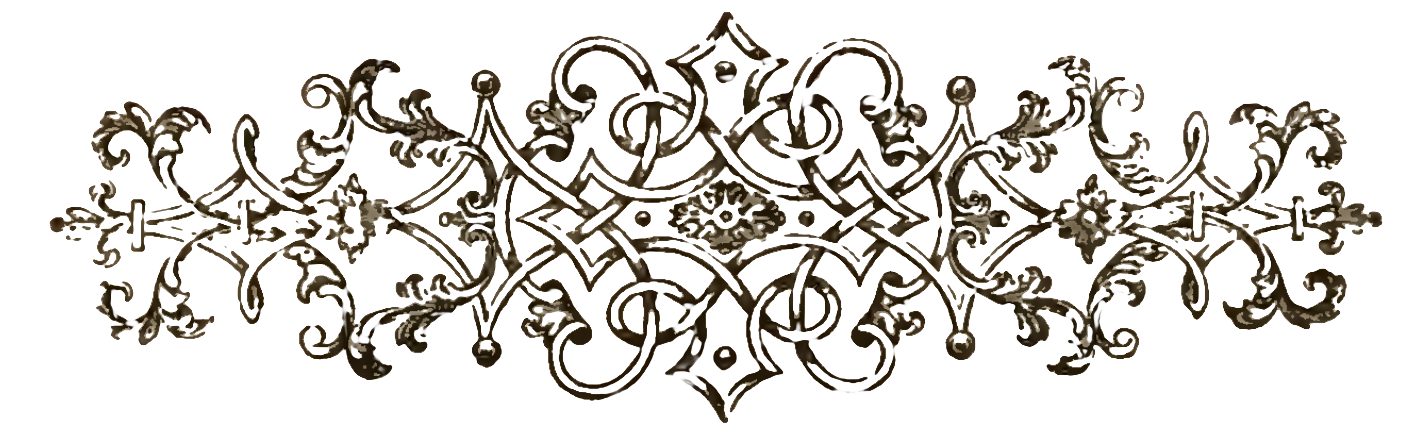
\includegraphics[width=15.5cm]{images/frontispiece.png}
\end{figure}

\end{document}
